
\section{Diagrama de comunicación entre procesos}

El diagrama de OndaPlay muestra cómo se comunican los
procesos que intervienen en el funcionamiento de esta
plataforma de streaming. En él se representan los
servicios que participan en las solicitudes del cliente,
la verificación de licencias y suscripciones, la consulta
del catálogo y el acceso al contenido audiovisual.

La Figura~\ref{fig:diagrama} presenta los procesos
de OndaPlay, sus interacciones y los actores externos
que participan en el sistema.

\begin{figure}[H]
    \centering
    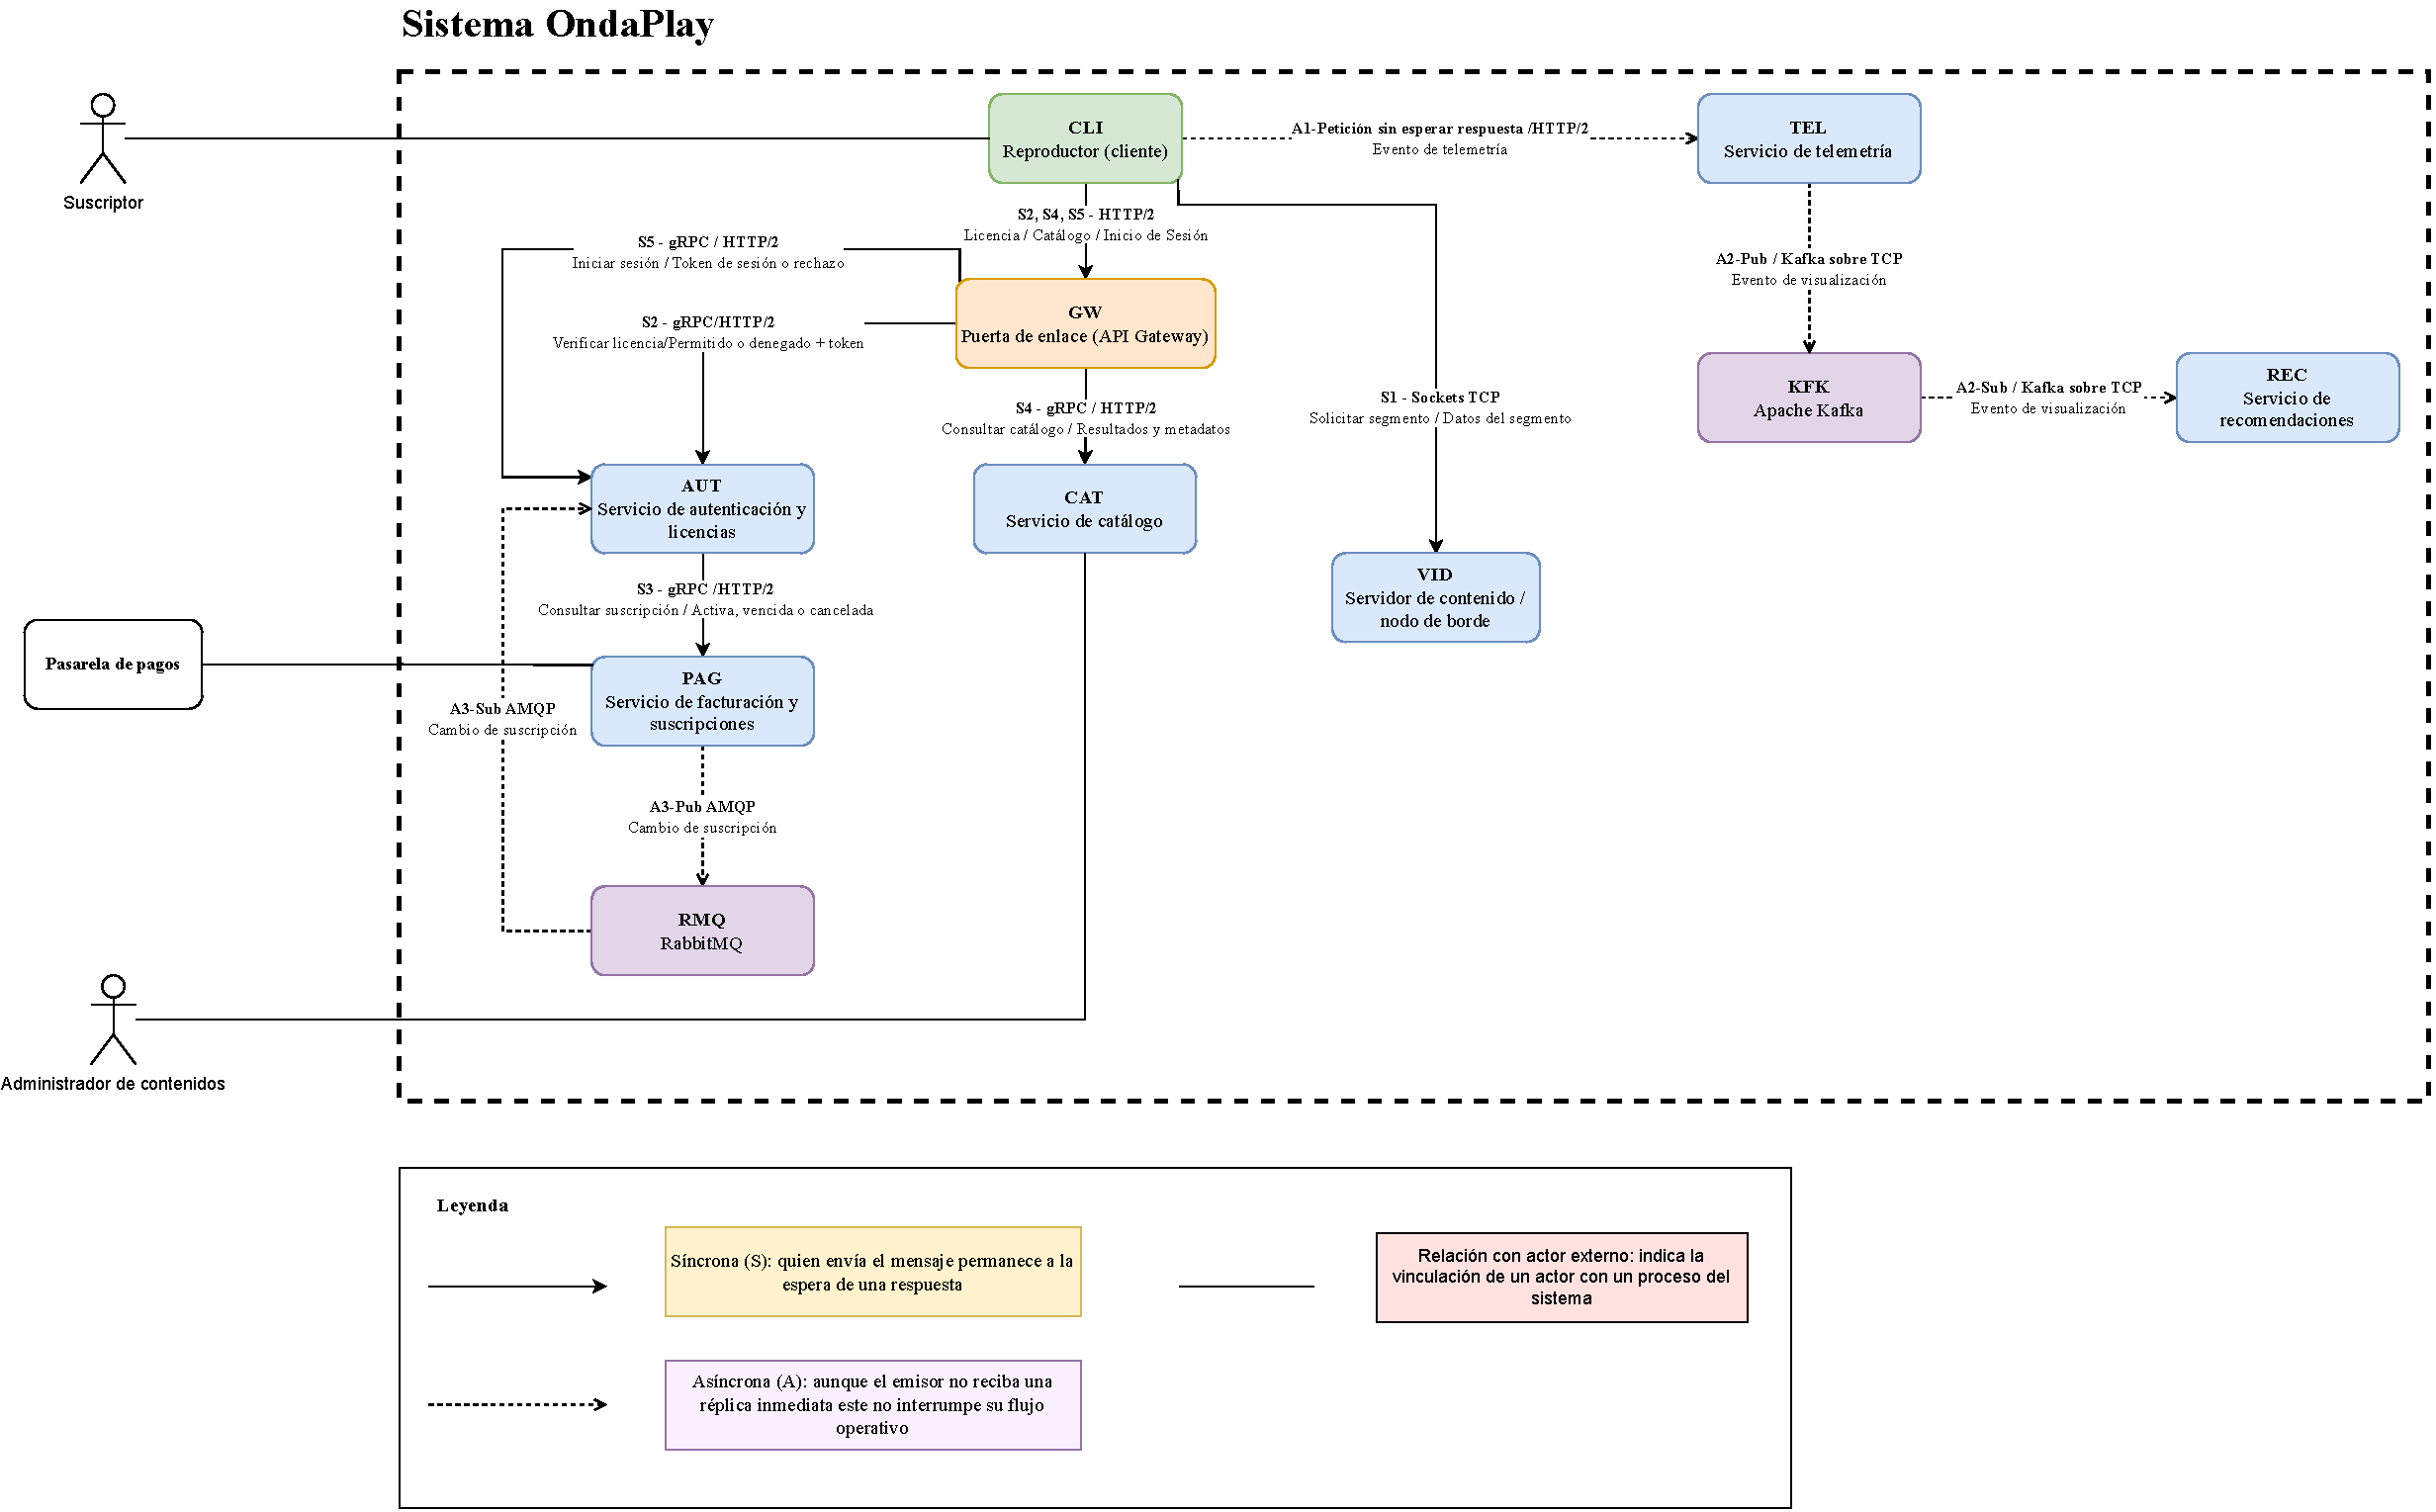
\includegraphics[width=\textwidth]{comunicacion}
    \caption{Comunicación entre los procesos y actores externos de OndaPlay}
    \label{fig:diagrama}
\end{figure}

\subsection{Componentes del sistema}

Los componentes se identifican mediante códigos que
permiten reconocerlos dentro del diagrama. CLI representa
al reproductor (cliente), desde el cual el suscriptor accede
a la plataforma, mientras que GW corresponde a la puerta de enlace que recibe y
dirige las solicitudes hacia los servicios internos.

AUT se encarga de la autenticación y las licencias, CAT representa el servicio de catálogo, VID corresponde
al servidor de contenido o nodo de borde, y PAG identifica al servicio de
facturación y suscripciones.

También se incluyen TEL, encargado de la telemetría, y
REC, representa al servicio de recomendaciones de contenido.
Para la comunicación asíncrona se utilizan KFK (Apache Kafka) y RMQ (RabbitMQ), estos permiten intercambiar
mensajes entre los procesos.

Fuera de la frontera del sistema se encuentran tres actores externos: Suscriptor (utiliza el reproductor), Administrador de contenidos
(interactúa con el catálogo) y Pasarela de pagos (se comunica con el servicio de facturación y suscripciones).

\subsection{Notación utilizada}

Las flechas indican la dirección en la que se envían
los mensajes entre los procesos. Se utilizan líneas
continuas para representar las comunicaciones síncronas,
en las que el emisor espera una respuesta antes de
continuar, y líneas discontinuas para las comunicaciones
asíncronas, en las que el emisor no necesita esperar
una respuesta inmediata.

Cada interacción se identifica con un código. La letra
S seguida de un número corresponde a una comunicación
síncrona, mientras que la letra A es utilizada para una
comunicación asíncrona. Junto a cada etiqueta se detallan los datos intercambiados, el mecanismo de
comunicación y el protocolo utilizado.

Las relaciones con los actores externos se representan mediante líneas continuas sin puntas de flecha en ninguno de sus extremos
y sin identificadores S o A (como los mencionados anteriormente). Estas líneas permiten distinguir la participación de los actores
de las comunicaciones entre los procesos internos de OndaPlay

\subsection{Lectura del diagrama}

En las comunicaciones síncronas representadas, S1 corresponde a la solicitud de segmentos de video desde el reproductor
(CLI) directamente al servidor de contenido (VID), sin pasar por la puerta de enlace (GW). Esta comunicación utiliza 
sockets TCP.

La interacción S2 corresponde a la comunicación entre GW y AUT para verificar las licencias. En S3, AUT consulta a PAG para comprobar el estado de la suscripción, 
mientras que S4 permite a GW solicitar información del catálogo a CAT.
Por su parte, S5 representa el inicio de sesión. La solicitud se envía desde CLI hacia GW y luego a AUT, 
donde se realiza la autenticación y se devuelve un token de sesión o un rechazo. Las interacciones S2, S3, S4 y S5 utilizan gRPC sobre HTTP/2.

En las comunicaciones asíncronas, A1 representa el envío de eventos de telemetría desde CLI hacia TEL. En A2, TEL publica eventos de visualización mediante Kafka (KFK), 
que posteriormente son consumidos por REC para generar recomendaciones.

Finalmente, A3 representa la comunicación desde PAG hacia AUT mediante RabbitMQ (RMQ), utilizada para informar los cambios en las suscripciones. Los mecanismos y protocolos de estas interacciones asíncronas se detallan en la Sección 4.